\documentclass[12pt]{article}
 
\usepackage[margin=1in]{geometry}
\usepackage{amsmath,amsthm,amssymb}
\usepackage{slashed, braket}
\usepackage{graphicx}
\usepackage{bbold}
 
\newcommand{\N}{\mathbb{N}}
\newcommand{\Z}{\mathbb{Z}}
 
\newenvironment{question}[2][Question]{\begin{trivlist}
\item[\hskip \labelsep {\bfseries #1}\hskip \labelsep {\bfseries #2.}]}{\end{trivlist}}
\newenvironment{questionpart}[2][Part]{\begin{trivlist}
\item[\hskip \labelsep \hskip \labelsep {\bfseries (#2)}]}{\end{trivlist}}

\newenvironment{solution}{\begin{proof}[Solution]}{\end{proof}}

\begin{document}

\title{Particle Physics HW 7}%replace X with the appropriate number
\author{Lucas Nestor}
 
\maketitle

\begin{question}{21.1}
Consider the decay $K\rightarrow2\pi$.
\end{question}

\begin{questionpart}{a}
What is the orbital angular momentum of the pions?
\end{questionpart}

\begin{solution}

We as always work in the rest frame of the decaying particle, meaning it has no orbital angular momentum. The $K$ is a spin-0 particle, so it has total angular momentum 0. The pions are also spin-0, so they cannot have any orbital angular momentum if the total angular momentum must also be 0.
\begin{equation*}
    \boxed{L_\pi=0}
\end{equation*}

\end{solution}

\begin{questionpart}{b}
What are the allowed isospin states of the two pions?
\end{questionpart}

\begin{solution}

As pions are bosons, their state must be symmetric. The symmetry for Clebsch Gordon coefficients is given by the equation below, where $I_1$ and $I_1$ are the isospin of the pions and $I$ is the isospin of the coupled state.
\begin{equation*}
    \text{Symmetry: }(-1)^{I_1+I_2-I}
\end{equation*}

Now, pions form an isospin triplet, so $I_1=I_2=1$. Thus,
\begin{equation*}
    \text{Symmetry: }(-1)^{2-I}
\end{equation*}

We see that we need $I$ to be an even number, i.e. $I=0,2$ but not $1$. We can also see this from the Clebsch-Gordon table for combining two spin-1 particles. The only states that are symmetric are $I=0$ and $I=2$.
\begin{equation*}
    \boxed{I=0,2}
\end{equation*}

\end{solution}

\begin{questionpart}{c}
Is $K^+\rightarrow\pi^+\pi^0$ allowed in weak decays, assuming only $|\Delta I|\leq 1$ is allowed?
\end{questionpart}

\begin{solution}

The $\pi^+$ has $I_3=+1$, while the $\pi^0$ has $I_3=0$. Looking at the Clebsch-Gordon table, we see that there are two possible states.
\begin{equation*}
    \ket{2,0}=\frac{1}{\sqrt{2}}(\ket{1,0}+\ket{0,1})=\frac{1}{\sqrt{2}}(\ket{\pi^+\pi^0}+\ket{\pi^0\pi^+})
\end{equation*}
\begin{equation*}
    \ket{1,0}=\frac{1}{\sqrt{2}}(\ket{1,0}-\ket{0,1})=\frac{1}{\sqrt{2}}(\ket{\pi^+\pi^0}-\ket{\pi^0\pi^+})
\end{equation*}

However, we said that we need $I=0$ or $I=2$, so only $I=2$ is valid here. Since $I=\frac{1}{2}$ for a $K$, we have $|\Delta I|=\frac{3}{2}$, so this is not allowed.
\begin{equation*}
    \boxed{|\Delta I|=\frac{3}{2}\text{, so this process is forbidden}}
\end{equation*}

\end{solution}

\begin{questionpart}{d}
Given the lifetimes and branching ratios for $K^+\rightarrow\pi^+\pi^0$ and $K^0\rightarrow\pi^+\pi^-$, calculate the ratio of the amplitudes for $|\Delta I|=\frac{3}{2}$ and $|\Delta I|=\frac{1}{2}$.
\end{questionpart}

\begin{solution}

We seek a ratio of amplitudes $\bra{f}S\ket{i}$ for these processes. The amplitudes are related to the partial decay rates. Here, $\phi$ is the phase space integral.
\begin{equation*}
    \Gamma(i\rightarrow f)=\phi |\bra{f}S\ket{i}|^2
\end{equation*}

Rearranging, we find the amplitude in terms of the partial decay rate.
\begin{equation*}
    \bra{f}S\ket{i}=\sqrt{\frac{\Gamma(i\rightarrow f)}{\phi}}
\end{equation*}

The partial decay rate is found from the branching ratio and total decay rate.
\begin{equation*}
    \Gamma(i\rightarrow f)=\text{BR}(i\rightarrow f) \Gamma(i)
\end{equation*}

Lastly, because $\Gamma(i)=\tau_i^{-1}$, we find the amplitude in terms of what we are given: the branching ratio and the lifetime.
\begin{equation*}
    \bra{f}S\ket{i}=\sqrt{\frac{\text{BR}(i\rightarrow f)}{\tau_i\phi}}
\end{equation*}

We saw from part (c) that the process $K^+\rightarrow\pi^+\pi^0$ has $|\Delta I|=\frac{3}{2}$. So now let's look at $K^0\rightarrow \pi^+ \pi^-$. The $\pi^-$ has $I_3=-1$. From the Clebsch-Gordon tables, we see that we have one possible state that is symmetric.
\begin{align*}
    \frac{1}{\sqrt{2}}(\ket{\pi^+\pi^-}&+\ket{\pi^-\pi^+})= \\
    &\frac{1}{\sqrt{2}}(\frac{1}{\sqrt{6}}\ket{2,0}+\frac{1}{\sqrt{2}}\ket{1,0}+\frac{1}{\sqrt{3}}\ket{0,0}+\frac{1}{\sqrt{6}}\ket{2,0}-\frac{1}{\sqrt{2}}\ket{1,0}+\frac{1}{\sqrt{3}}\ket{0,0}) \\
    &= \frac{1}{\sqrt{3}}\ket{2,0}+\sqrt{\frac{2}{3}}\ket{0,0}
\end{align*}

We see that it has a $|\Delta I|=\frac{3}{2}$ and $|\Delta I|=\frac{1}{2}$ component. We know that the $|\Delta I|=\frac{1}{2}$ will dominate, so we can suppress the other one.

Alright, we can put it all together now.
\begin{equation*}
    \left|\Delta I=\frac{3}{2}\right|\rightarrow \bra{\pi^+\pi^0}S\ket{K^+}=\sqrt{\frac{\text{BR}(K^+\rightarrow\pi^+\pi^0)}{\tau_{K^+}\phi}}
\end{equation*}
\begin{align*}
    \left|\Delta I=\frac{1}{2}\right|\rightarrow \bra{\pi^+\pi^-}S\ket{K^0}&=\sqrt{\frac{2}{3}}\bra{0,0}S\ket{K^0} \\ 
    \bra{0,0}S\ket{K^0} &= \sqrt{\frac{3\text{BR}(K^0\rightarrow\pi^+\pi^-)}{2\tau_{K^0}\phi}}
\end{align*}

Now we take the ratio of these.
\begin{align*}
    R=\frac{\bra{\pi^+\pi^0}S\ket{K^+}}{\bra{0,0}S\ket{K^0}}&=\sqrt{\frac{\text{BR}(K^+\rightarrow\pi^+\pi^0)}{\tau_{K^+}\phi}}/\sqrt{\frac{3\text{BR}(K^0\rightarrow\pi^+\pi^-)}{2\tau_{K^0}\phi}} \\
    &= \sqrt{\frac{2\tau_{K^0}\text{BR}(K^+\rightarrow\pi^+\pi^0)}{3\tau_{K^+}\text{BR}(K^0\rightarrow\pi^+\pi^-)}}
\end{align*}

And we plug in the numbers given.
\begin{equation*}
    \boxed{R=0.038}
\end{equation*}

\end{solution}

\newpage

\begin{question}{21.2}
Find the mass of the $\Delta^{++}$ and $K^{*+}$ from the Dalitz plot given.
\end{question}

\begin{solution}

This is essentially a relativistic collision problem. We have an incoming particle at a stationary target in the lab frame, we will describe this collision by $12\rightarrow 34$.

We are given a few things: $E_{1,\text{lab}}$, $m_1$, $m_2$, $m_4$, and $E_{4,\text{CM}}$, and we seek $m_3$. We will solve this by considering 4-momentum conservation in both frames.
\begin{align*}
    p_1^\mu+p_2^\mu=p_3^\mu+p_4^\mu
\end{align*}

In the CM frame, we have $\vec{p}_3=-\vec{p}_4$. Thus,
\begin{align*}
    {\vec{p}_3}^2={\vec{p}_4}^2\rightarrow E_3^2-m_3^2=E_4^2-m_4^2
\end{align*}

We know everything except $E_3$. To get that, we'll consider conservation of energy.
\begin{equation*}
    E_3+E_4=E_{CM}=\sqrt{s}
\end{equation*}

Meanwhile,
\begin{equation*}
    s=(P_{1,\text{lab}}^\mu+P_{2,\text{lab}}^\mu)^2=P_1^2+P_2^2+2P_1P_2=m_1^2+m_2^2+2E_{1,\text{lab}}m_2
\end{equation*}

Putting it all together,
\begin{align*}
    (\sqrt{s}-E_4)^2-m_3^2&=E_4^2-m_4^2
\end{align*}

Or,
\begin{align*}
    m_3^2=s+m_4^2-2E_4\sqrt{s}
\end{align*}

Now we can plug in the numbers for the two processes. For $K^+p\rightarrow K^0\Delta^{++}$, we have $m_4=0.498$ GeV and $E_4=1.0549$ GeV. Our center of mass energy $s$ is $s=m_p^2+m_{K^+}^2+2E_{1,\text{lab}}m_p=6.75$ GeV. This gives us $m_{\Delta^{++}}=1.23$ GeV.

For the $K^+p\rightarrow K^{*+}p$, we have $m_4=0.938$ GeV and $E_4=1.3154$. This gives us $m_{K^{*+}}=0.89$ GeV.

In summary,
\begin{equation*}
    \boxed{m_{\Delta^{++}}=1.23\text{ GeV}\qquad m_{K^{*+}}=0.89\text{ GeV}}
\end{equation*}

\end{solution}

\newpage

\begin{question}{22.1}
Find the generators of $SU(2)$ in the $I=\frac{3}{2}$ representation. Show that these matrices satisfy the $SU(2)$ Lie algebra.
\end{question}

\begin{solution}

Because the states $\ket{t_3}$ are labelled by eigenvalues of $T_3$, finding that matrix is trivial.
\begin{equation*}
    \boxed{T_3=\begin{pmatrix}
        \frac{3}{2} & 0 & 0 & 0 \\
        0 & \frac{1}{2} & 0 & 0 \\
        0 & 0 & -\frac{1}{2} & 0 \\
        0 & 0 & 0 & -\frac{3}{2}
    \end{pmatrix}}
\end{equation*}

Next, we can find $T_\pm$ easily since $(T_\pm)_{t_3t_3'}=\sqrt{I(I+1)-t_3(t_3\pm1)}\delta_{t_3,t_3'\pm1}$. We are in the $I=\frac{3}{2}$ representation.
\begin{equation*}
    T_+=\begin{pmatrix}
        0 & \sqrt{3} & 0 & 0 \\
        0 & 0 & 2 & 0 \\
        0 & 0 & 0 & \sqrt{3} \\
        0 & 0 & 0 & 0
    \end{pmatrix}
\end{equation*}
\begin{equation*}
    T_-=\begin{pmatrix}
        0 & 0 & 0 & 0 \\
        \sqrt{3} & 0 & 0 & 0 \\
        0 & 2 & 0 & 0 \\
        0 & 0 & \sqrt{3} & 0
    \end{pmatrix}
\end{equation*}

We can use these to get $T_1$ and $T_2$ since $T_\pm=T_1\pm i T_2$.
\begin{align*}
    T_1&=\frac{1}{2}(T_++T_-) \\
    T_2&=\frac{1}{2i}(T_+-T_-)=\frac{i}{2}(T_--T_+)
\end{align*}

Plugging in our matrices for $T_+$ and $T_-$ gives us what we want.
\begin{equation*}
    \boxed{T_1=\frac{1}{2}\begin{pmatrix}
        0 & \sqrt{3} & 0 & 0 \\
        \sqrt{3} & 0 & 2 & 0 \\
        0 & 2 & 0 & \sqrt{3} \\
        0 & 0 & \sqrt{3} & 0
    \end{pmatrix}}
\end{equation*}
\begin{equation*}
    \boxed{T_2=\frac{i}{2}\begin{pmatrix}
        0 & -\sqrt{3} & 0 & 0 \\
        \sqrt{3} & 0 & -2 & 0 \\
        0 & 2 & 0 & -\sqrt{3} \\
        0 & 0 & \sqrt{3} & 0
    \end{pmatrix}}
\end{equation*}

Now we want to check the commutation relations of these matrices without explicitly computing them.
\begin{align*}
    [T_i,T_j]_{t_3t_3'}&=\sum_x\bra{t_3}T_i\ket{x}\bra{x}t_j\ket{t_3'}-\bra{t_3}T_j\ket{x}\bra{x}t_i\ket{t_3'} \\
    &= \bra{t_3}T_i \mathbb{1} T_j - T_j \mathbb{1} T_i \ket{t_3'} \\
    &= \bra{t_3}[T_i,T_j]\ket{t_3'}
\end{align*}

We know the generators of the group follow $[T_i,T_j]=i\epsilon_{ijk} T_k$, so we plug that in.
\begin{align*}
    [T_i,T_j]_{t_3t_3'}=\bra{t_3}i\epsilon{ijk}T_k\ket{t_3'}=i\epsilon_{ijk}(T_k)_{t_3t_3'}
\end{align*}

Or,
\begin{equation*}
    \boxed{[T_i,T_j]=i\epsilon_{ijk}T_k}
\end{equation*}

\end{solution}

\newpage

\begin{question}{23.1}
Given the generators of $SU(3)$ satisfy the Lie algebra $[T_a,T_b]=if_{abc}T_c$, answer the following questions.
\end{question}

\begin{questionpart}{a}
Show the conjugate representation generators $\overline{T}_a\equiv-T_a^T$ satisfy the $SU(3)$ algebra.
\end{questionpart}

\begin{solution}
This is straightforward from just computing the commutators.
\begin{align*}
    [\overline{T}_a,\overline{T}_b]&=[-T_a^T,-T_b^T]=T_a^TT_b^T-T_b^TT_a^T=-[T_a, T_b]^T\\
    &=-if_{abc}T_c^T=if_{abc}(-T_c^T)=if_{abc}\overline{T}_c
\end{align*}

We see it follows the same algebra.
\begin{equation*}
    \boxed{[\overline{T}_a,\overline{T}_b]=\overline{T}_c }
\end{equation*}

\end{solution}

\begin{questionpart}{b}
Show the adjoint representation generators $(F_a)_{bc}\equiv-if_{abc}$ satisfy the $SU(3)$ algebra using the Jacobi identity.
\end{questionpart}

\begin{solution}

We start by plugging in the commutation relations to the Jacobi identity. I'll do it term by term because it will get messy.
\begin{align*}
    [[T_a,T_b],T_c]&=if_{abx}[T_x,T_c]=-f_{abx}f_{xcz} \\
    [[T_b,T_c],T_a]&=if_{bcx}[T_x,T_a]=-f_{bcx}f_{xaz} \\
    [[T_c,T_a],T_b]&=if_{cax}[T_x,T_b]=-f_{cax}f_{xbz}
\end{align*}

Putting it all together,
\begin{equation*}
    f_{abx}f_{xcz}+f_{bcx}f_{xaz}+f_{cax}f_{xbz}=0
\end{equation*}

Now we do a bunch of index shuffling until we get the form we want. First we move the left term to the RHS of the equation. We also make the substitution $c\rightarrow x$ so that $x$ and $z$ are the two free indices on both sides.
\begin{equation*}
    f_{bxy}f_{yaz}+f_{xay}f_{ybz}=-f_{abc}f_{cxz}
\end{equation*}

The reason we do this is now we can write the RHS as $-f_{abc}f_{cxz}$=$-if_{abc}(F_c)_{xz}$. We can start to see the Lie algebra develop. Now on the LHS we want to swap around the first two indices for a few terms. Doing this gives us $f_{abc}=-f{bac}$.
\begin{align*}
    -f_{bxy}f_{ayz}+f_{axy}f_{byz}&=(-if_{bxy})(-if_{ayz})-(-if_{axy})(-if_{byz}) =-[F_a,F_b]_{xz}
\end{align*}

Putting it all together, the minus sign cancels and we get exactly what we want
\begin{equation*}
    \boxed{[F_a,F_b]=if_{abc}F_c}
\end{equation*}
\end{solution}

\begin{questionpart}{c}
Find all states in the multiplet with the highest weight state of $t_3=\frac{3}{2}$ and $y=1$. Draw the weight diagram with the charge of each state.
\end{questionpart}

\begin{solution}

Since this is the highest weight state, it is clear to see that this forms an isospin quadruplet. We also see there are three generators that will yield 0.
\begin{equation*}
    T_+\ket{\frac{3}{2},1}=V_+\ket{\frac{3}{2},1}=U_-\ket{\frac{3}{2},1}=0 
\end{equation*}

We now seek to see what sort of U-spin and V-spin multiplet this state is a part of. We will start with U-spin.
\begin{equation*}
    U_3\ket{\frac{3}{2},1}=(\frac{3}{4}Y-\frac{1}{2}T_3)\ket{\frac{3}{2},1}=0
\end{equation*}

Since this is the lowest U-spin weight state of this multiplet, we determine that it forms a singlet. Now we check V-spin.
\begin{equation*}
    V_3\ket{\frac{3}{2},1}=(\frac{3}{4}Y+\frac{1}{2}T_3)\ket{\frac{3}{2},1}=\frac{3}{2}
\end{equation*}

This is the highest V-spin weight state, so this must be a quadruplet. Thus, we can start to fill out the weight diagram with what we know currently.

\begin{figure}[h!]
    \centering
    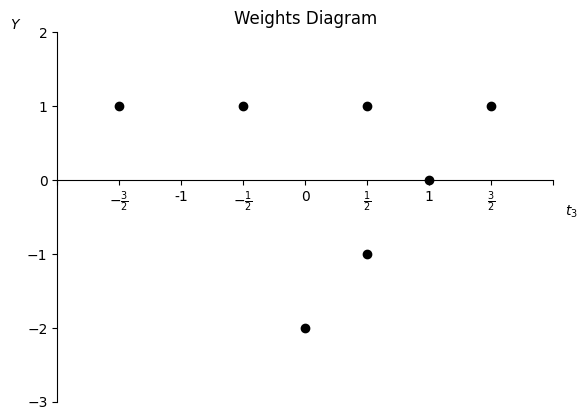
\includegraphics[width=0.5\linewidth]{weights_diagram1.png}
\end{figure}

Now let's check the isospin of the state $\ket{1,0}$, specifically if it is the highest weight state.
\begin{equation*}
    T_+\ket{1,0}=T_+V_+\ket{\frac{3}{2},1}=[T_+,V_+]\ket{\frac{3}{2},1}=0
\end{equation*}

Thus, this is a highest weight state, and it forms an isospin triplet. Lastly, we will look at the U-spin of the state $\ket{0,-2}$.
\begin{equation*}
    U_-\ket{0,-2}=U_-V_+^3\ket{\frac{3}{2},1}=[U_-,V_+^3]\ket{\frac{3}{2},1}=0
\end{equation*}

Thus, $\ket{0,-2}$ is the lowest weight state of a U-spin multiplet. We can see that it is a quadruplet.
\begin{equation*}
    U_3\ket{0,-2}=(\frac{3}{4}Y-\frac{1}{2}T_3)\ket{0,-2}=-\frac{3}{2}
\end{equation*}

So our weight diagram is (almost) fully filled out.

\begin{figure}[h!]
    \centering
    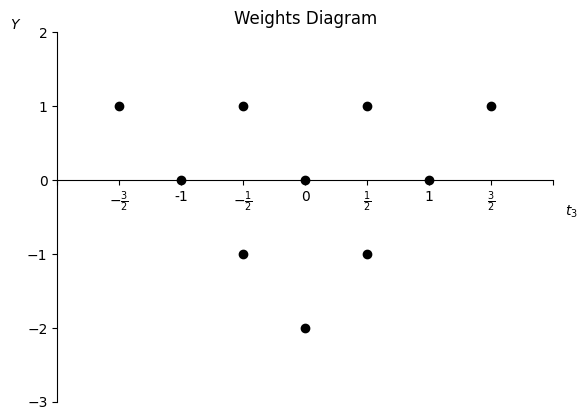
\includegraphics[width=0.5\linewidth]{weights_diagram2.png}
\end{figure}

\newpage

Our last task is to check the uniqueness of the middle state. Let's assume the middle state is a superposition of two states, $\ket{a}$ and $\ket{b}$. Then we will approach it from two directions.
\begin{equation*}
    V_-\ket{\frac{1}{2},1}=a\ket{a}+b\ket{b}
\end{equation*}
\begin{equation*}
    U_+\ket{\frac{1}{2},-1}=a'\ket{a}+b'\ket{b}
\end{equation*}

We can find the norm of these states.
\begin{equation*}
    \bra{\frac{1}{2},1}V_+V_-\ket{\frac{1}{2},1}=\bra{\frac{1}{2},1}[V_+,V_-]\ket{\frac{1}{2},1}=2\bra{\frac{1}{2},1}V_3\ket{\frac{1}{2},1}=2
\end{equation*}
\begin{equation*}
    \bra{\frac{1}{2},-1}U_-U_+\ket{\frac{1}{2},-1}=\bra{\frac{1}{2},-1}[U_-,U_+]\ket{\frac{1}{2},-1}=2\bra{\frac{1}{2},-1}U_3\ket{\frac{1}{2},-1}=2
\end{equation*}

Thus, $a^2+b^2=a'^2+b'^2=2$. Now we notice that $[U_+,V_-]=T_-$, so $[U_+,V_-]=T_-=0$.
\begin{align*}
    (U_+V_--V_-U_+-T_-)\ket{1,0}=0 \\
    2U_+\ket{\frac{1}{2},-1}-V_-\ket{\frac{1}{2},1}-\sqrt{2}\ket{a}=0 \\
    2 (a'\ket{a}+b'\ket{b})-(a\ket{a}+b\ket{b})-\sqrt{2}\ket{a}=0 \\
    (2a'-a-\sqrt{2})\ket{a}+(b'-b)\ket{b}=0
\end{align*}

We take $\ket{a}$ and $\ket{b}$ to be orthogonal, so this requires $2a'-a-\sqrt{2}=0$ and $b'-b=0$. Solving these 4 equations yields us the coefficients.
\begin{equation*}
    b'=b=0\qquad a'=a=\sqrt{2}
\end{equation*}

Thus, we see that the central state is unique.

The last thing we need to do is write the charge for each state with $Q=T_3+\frac{Y}{2}$. You can see that this equation defines a line $Y=2(Q-T_3)$, i.e. lines with negative slope have a constant charge. So, we can label the charges of each state. See the diagram below.

\begin{figure}[t]
    \centering
    \boxed{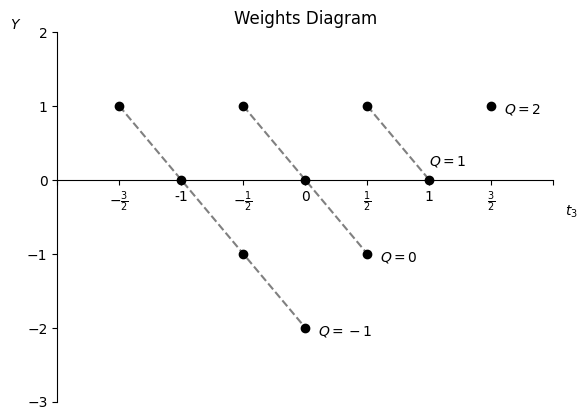
\includegraphics{weights_diagram3.png}}
\end{figure}

\end{solution}

\end{document}